\documentclass{asaproc}

\usepackage{amsmath}
\usepackage{times}
\usepackage{graphicx}
\usepackage{bbm}



%For figures and tables to stretch across two columns
%use \begin{figure*} \end{figure*} and
%\begin{table*}\end{table*}
% please place figures & tables as close as possible
% to text references


\newcommand{\be}{\begin{equation}}
\newcommand{\ee}{\end{equation}}

 \title{Rounded Data}

%input all authors' names

\author{Robert Espinoza}







\begin{document}

\maketitle


\begin{abstract}
In this case study we will be examining UV index data, which is rounded data to the nearest whole number.  It is unreasonable to assume the rounded data is a random sample from a normal distribution, but it would be reasonable to assume the unobserved unrounded measurements are independently distributed from a normal distribution with mean $\mu$ and variance $\sigma^2$.  We analyze the data in two different models, model (a) does not take into account the original $x_{1},..,x_{10}$ unobserved unrounded data in the joint posterior distribution, and model (b) takes into account does take into account the $x_{1},..,x_{10}$ in the joint posterior distribution.  In both models we assume a non-informative prior $(\mu,\sigma^2)\propto \frac{1}{\sigma^2}$.  The rounded data is as follows: 7, 6, 7, 5, 5, 3, 6, 5, 4, 3.
\end{abstract}


\section{Model (a)}

First we determine the probability of the individual observations given our parameters of interest $(\mu,\sigma^2)$.

\begin{equation*}
Pr(y_{i} | \mu,\sigma^2) = \Phi(\frac{y_{i}+0.5-\mu}{\sigma}) - \Phi(\frac{y_{i}-0.5-\mu}{\sigma})
\end{equation*}

The joint posterior distribution for model (a) is as follows:
\begin{align*}
p(\mu,\sigma^2 | \mathbf{y}) &\propto p(\mu,\sigma^2)p(\mathbf{y} | \mu,\sigma^2) \\
&= \frac{1}{\sigma^2}\prod_{i=1}^{10}[\Phi(\frac{y_{i}+0.5-\mu}{\sigma}) - \Phi(\frac{y_{i}-0.5-\mu}{\sigma})]
\end{align*}

We are now interested in sampling from the joint posterior distribution, which will be executed by an grid approximation sampling algorithm.  The sketch of the algorithm is as follows:\\\\
1. Generate a grid of points for $\mu$ and $\sigma^2$, and contour values. \\
2. Determine the target posterior distribution.\\
3. Generate a contour plot with the grid points and posterior distribution. \\
4. Normalize $\mu$ marginal density. \\
5. Sample $\mu$ indices from the $\mu$ grid of points with the normalized $\mu$ density. \\
6.  Generate $\mu$ sample from sampled indices at the $\mu$ grid of points. \\
7. Generate $\sigma^2$ sample at the $\sigma^2$ grid of points with posterior density probabilities at the sampled $\mu$ indices.  \\

The above algorithm will provide us with an appropriate sample of $(\mu, \sigma^2)$

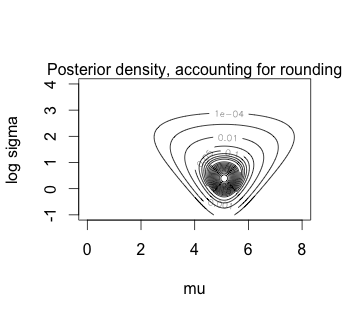
\includegraphics[scale=.5]{/Users/cowabungadood/Desktop/ams207/Midterm/contourpost.png}
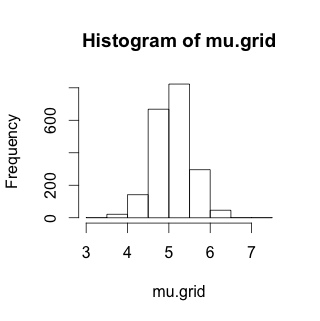
\includegraphics[scale=.5]{/Users/cowabungadood/Desktop/ams207/Midterm/Rplot01.png}
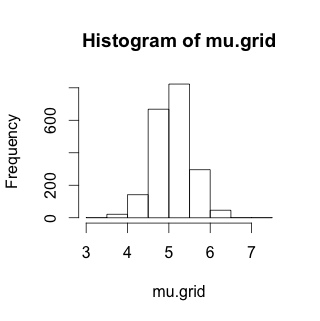
\includegraphics[scale=.5]{/Users/cowabungadood/Desktop/ams207/Midterm/Rplot02.png}

\section{Model (b)}

The second model we will take into account is a posterior distribution with the unobserved unrounded measurements $x_{1},..,x_{10}$ as random variables.  Since the data involves $x_{i}$ covariates in the posterior, we will require an inclusion distribution to derive the complete likelihood of the data. The posterior distribution is as follows:


\begin{align*}
p(\mu,\sigma^2, \mathbf{x} | \mathbf{y}, I) &\propto p(\mu,\sigma^2)p(\mathbf{y} | \mu,\sigma^2)p(I | \mathbf{x}, \mathbf{y})p(\mathbf{x} | \mu, \sigma^2) \\
&= \prod_{i=1}^{10}[\Phi(\frac{y_{i}+0.5-\mu}{\sigma}) - \Phi(\frac{y_{i}-0.5-\mu}{\sigma})] \\
&\mathbbm{1}_{y_{i}-0.5<x_{i}<y_{i}+0.5}(\sigma^2)^{-6}\\
&\exp(-\frac{1}{2\sigma^2}\sum_{i=1}^{10}(x_{i}-\mu)^2)\\
\end{align*}

In order to sample from this particular joint posterior distribution we will us a Markov Chain Monte Carlo sampling algorithm.  We will utilize a Gibbs sampler with a random walk Metropolis Hastings algorithm to sample $(\mu, \sigma^2, x_{1},..,x_{10})$.  The following are the full conditional distributions that will be used in the Gibbs sampling algorithm:

\begin{equation*}
p(x_{i}|y_{i},\mu,\sigma^2,I) \propto \mathbbm{1}_{y_{i}-0.5<x_{i}<y_{i}+0.5}\exp(\frac{-1}{2\sigma^2}(x_{i}-\mu)^2)
\end{equation*}

\begin{align*}
p(\mu|\mathbf{y},\mathbf{x},\sigma^2) &\propto \prod_{i=1}^{10}[\Phi(\frac{y_{i}+0.5-\mu}{\sigma}) - \Phi(\frac{y_{i}-0.5-\mu}{\sigma})]\\&\exp(\frac{-5}{\sigma^2}(\mu-x_{i})^2)
\end{align*}

\begin{align*}
p(\sigma^2|\mathbf{y},\mathbf{x},\mu) &\propto \prod_{i=1}^{10}[\Phi(\frac{y_{i}+0.5-\mu}{\sigma}) - \Phi(\frac{y_{i}-0.5-\mu}{\sigma})]\\&(\sigma^2)^{-6}\exp(\frac{-1}{2\sigma^2}\sum_{i=1}^{10}(x_{i}-\mu)^2)
\end{align*}

The sketch of the Gibbs sampling algorithm is as follows:\\\\
1. set $\mu_0$ and $\sigma^2_0$ starting values. \\
2. draw $x_1$ though $x_10$ using the full conditional of each of the $x_{i}$ and use necessary current values to update, save draws as current values. \\
3. draw $\mu$ using the full conditional of $\mu$ which is approximated using a random walk Metropolis Hastings step using necessary current values to update, and save as current value. \\
4. draw a $\sigma^2$ using the full conditional of $\sigma^2$ which is approximated using a random walk Metropolis Hastings step using necessary current values to update, and save as current value. \\
5. burn-in and thin draws to eliminate correlation between draws. \\
6. repeat the above steps until necessary number of iterations has been completed. \\


The above algorithm will provide samples for $(x_{1},...,x_{10}, \mu, \sigma^2)$.

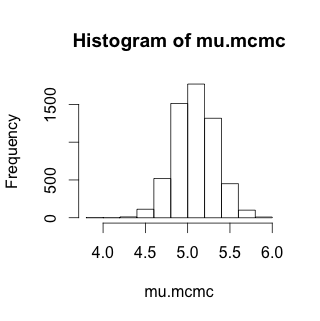
\includegraphics[scale=.5]{/Users/cowabungadood/Desktop/ams207/Midterm/Rplot04.png}
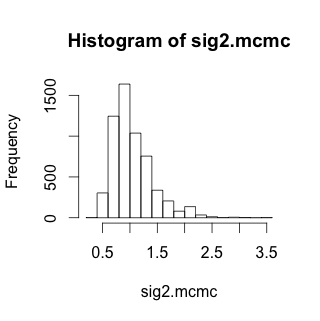
\includegraphics[scale=.5]{/Users/cowabungadood/Desktop/ams207/Midterm/Rplot03.png}



\section{Model Comparison}
Below are summary statistics of model (a): 
\begin{center}
    \begin{tabular}{ | l | l | l | p{5cm} |}
    \hline
    parameter & Mean & $95\%$ Posterior Interval \\ \hline
    $\mu$ & 5.09 & [4.18, 5.98]   \\ \hline
    $\sigma^2$ & 1.95 & [0.743, 4.65] \\ \hline
     \end{tabular}
\end{center}

Below are the summary statistics of model (b):

\begin{center}
    \begin{tabular}{ | l | l | l | p{5cm} |}
    \hline
    Parameter & Mean & $95\%$ Posterior Interval \\ \hline
    $\mu$ & 5.08 & [4.61, 5.57]   \\ \hline
    $\sigma^2$ & 1.04 & [0.519, 2.04] \\ \hline
    $x_{1}$ & 6.84 & [6.51, 7.43] \\ \hline
    $x_{2}$ & 5.92 & [5.51, 6.45] \\ \hline
    $x_{3}$  & 6.84 & [6.51, 7.43] \\ \hline
    $x_{4}$  & 5.01 & [4.53, 5.47] \\ \hline
    $x_{5}$  & 5.01 & [4.52, 5.47] \\ \hline
    $x_{6}$  & 3.16 & [2.57, 3.49] \\ \hline
    $x_{7}$  & 5.92 & [5.52, 6.45] \\ \hline
    $x_{8}$  & 5.01 & [4.52, 5.47] \\ \hline
    $x_{9}$  & 4.09 & [3.55, 4.48] \\ \hline
    $x_{10}$  & 3.15 & [2.58, 3.48] \\ \hline
    \end{tabular}
\end{center}

The confidence intervals of model (a) versus model (b) for $\mu$ and $\sigma^2$ are more tightly bounded for model2.  This is possibly due to the fact that we introduced the inclusion parameter and unknown unrounded random variables into the joint posterior.  The mean for $\sigma^2$ for model (b) was noticeably lower than model (a), which may be due to an error in my analysis, or maybe be due to the fact that with the addition of the $x_{i}$ random variables, it improved the estimate of the $\sigma^2$, which may indicate that the true $\sigma^2$ is near 1.  With the tighter bounds around $\mu$ and $\sigma^2$, model (b) seems to be more robust, and should be the model to work with for future analysis. The DIC for model (a) is 41.35 and the DIC for model (b) i s40.75, therefore the DIC agrees with our assumption that model (b) is a better model. 


\begin{references}
{\footnotesize
\itemsep=3pt




\item Gelman A., Robert C, Chopin N., Rousseau J.(2013),  ``Bayesian Data Analysis''

}
\end{references}


\end{document}

